%%%%%%%%%%%%%%%%%%%%%%%%%%%%%%%%%%%%%%%%%%%%%%%%%%%%%%%%%%%%%%%%%%%%%%%%%%%%%%%%
%2345678901234567890123456789012345678901234567890123456789012345678901234567890
%        1         2         3         4         5         6         7         8

\documentclass[letterpaper, 10 pt, conference]{ieeeconf}  % Comment this line out if you need a4paper
\usepackage{url}
\usepackage{cite}
% The following packages can be found on http:\\www.ctan.org
\usepackage{graphics} % for pdf, bitmapped graphics files
%\usepackage{graphicx} % for pdf, bitmapped graphics files
\usepackage{epsfig} % for postscript graphics files
\usepackage{mathptmx} % assumes new font selection scheme installed
\usepackage{times} % assumes new font selection scheme installed
\usepackage{amsmath} % assumes amsmath package installed
\usepackage{amssymb}  % assumes amsmath package installed
\usepackage{gensymb}
\usepackage{epstopdf}
\usepackage[]{units}
%\usepackage{subscript}
\usepackage{color}
\usepackage{verbatim}
\usepackage{psfrag}
\bibliographystyle{IEEEtran}
\usepackage{textcomp}
\usepackage{graphicx}
\usepackage{caption}
\usepackage{subcaption}
%\usepackage{algpseudocode}
\usepackage{algorithmic}
\usepackage[Pseudocode]{algorithm}
\usepackage{todonotes}
\usepackage{bm}
\usepackage{empheq}
\usepackage{pgfplots}
\usepackage{multirow}
%\usepackage[table,xcdraw]{xcolor}

%% TO USE HYPERREF (BUG IN IEEE style) (REMOVE BEFORE PUBLICATION)
\makeatletter
\let\NAT@parse\undefined
\makeatother
\usepackage{hyperref}

\pdfminorversion=4
%\documentclass[a4paper, 10pt, conference]{ieeeconf}      % Use this line for a4 paper

\IEEEoverridecommandlockouts                              % This command is only needed if 
% you want to use the \thanks command

\overrideIEEEmargins                                      % Needed to meet printer requirements.

% See the \addtolength command later in the file to balance the column lengths
% on the last page of the document

\title{\LARGE \bf
	Dynamic Markers: Optimal control point configurations for homography and pose estimation
}


\author{Raul Acuna$^{1}$, and Volker Willert$^{1}$% <-this % stops a space
	\thanks{*This work was sponsored by the German Academic Exchange Service (DAAD) and the Becas Chile doctoral scholarship.}% <-this % stops a space
	\thanks{$^{1}$These authors are within the Institute of Automatic Control and Mechatronics, Technische Universit{\"a}t Darmstadt, Germany.{\tt\small (racuna, vwillert)}{\tt\small @rmr.tu-darmstadt.de}}}

\begin{document}
	\maketitle
	\thispagestyle{empty}
	\pagestyle{empty}
	%%%%%%%%%%%%%%%%%%%%%%%%%%%%%%%%%%%%%%%%%%%%%%%%%%%%%%%%%%%%%%%%%%%%%%%%%%%%%%%%
	\begin{abstract}
		In this paper, we shed some light on the influence of control points on the accuracy of space resectioning methods, e.g. used by a fiducial marker for pose estimation. More precisely, we propose a gradient descent optimization method to find optimal configurations of control points for the tasks of homography estimation and subsequent planar pose estimation from a number of $n \geq 4$ noisy point correspondences. We obtain optimal configurations by minimizing the first order perturbed solution of the direct linear transform (DLT) algorithm which is equivalent to minimizing the condition number of the data matrix. This method guarantees points configurations which maximize the robustness of the DLT homography estimation.
		Furthermore, a statistical evaluation is presented verifying that this optimal control points configurations also increase the performance of very accurate state of the art homography as well as pose estimation methods, like IPPE and EPnP, including the iterative minimization of the reprojection error MRE which is the most accurate algorithm and serves as golden standard. Finally, we provide a tradeoff between optimal configuration against number of control points.
	\end{abstract}
	
	%(3D-2D)
	%(that minimize the sensitivity to noise)
	%(condition number of the data matrix in the)
	%(for the minimal number of four control points sets (also 5 and 6?) found)
	%These results shed some light on the influence of the control model points on the accuracy %of space resectioning methods, which has been an open problem in the literature so far.
	%(not only for the DLT transform but as well for other homography estimation methods).
	%(Finally, looking at the statistics of the point configurations, we derive new rotation and %scaling invariant coordinate normalizations $T(H)$ as a function of the homography itself.
	
	%%%%%%%%%%%%%%%%%%%%%%%%%%%%%%%%%%%%%%%%%%%%%%%%%%%%%%%%%%%%%%%%%%%%%%%%%%%%%%%%
	\section{INTRODUCTION}
	
	\textcolor{red}{We need a figure that shows the geometry of the overall task and the movement of the points ...}
	
	%\subsection{Motivation}
	%Why?
	Space resectioning, homography estimation and the PnP problem are some of the most researched topics in the fields of Computer Vision and Photogrammetry. Even though the research on these areas has been wide, there is a surprisingly lack of information regarding the effect of the 3D control point configurations on the accuracy and stability of the estimation methods.
	
	%What? For Whom?
	It is clear from the literature (As will be shown in Chapter \ref{state_of_the_art}) that the control points configurations are relevant. First, it is widely accepted that increasing the number of control points increases the accuracy of the methods in presence of noise (refs?). Second, the spatial configuration of the points affects the estimation. In several studies when simulations are performed to compare methods, great care is given to possible singular points configurations, such as non centered data or near planar cases which are singularities or degenerate cases for certain estimation methods. Additionally, in homography estimation and planar pose estimation methods based on homography it is important to include a normalization step of both the control points and image points. 
	
	\begin{figure}[t]
		\begin{center}
			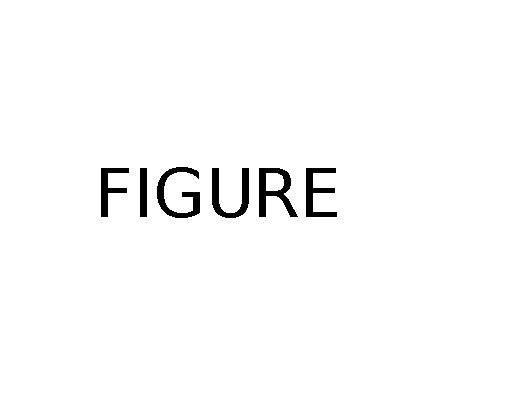
\includegraphics[width=\columnwidth]{img/intro_figure.pdf}
			\caption{\label{fig:intro_figure} FILL OUT DESCRIPTION.}
		\end{center}
	\end{figure}
	
	However, none of the above give an answer to a simple question: 
	
	\textit{Is there a n-point configuration which can increase the likelihood for a space resectioning method to find the best possible solution?}
	
	Many more questions are also connected to this main one:
	
	\begin{itemize}
		\item May a well conditioned n-points configuration be better than a (an ill-conditioned or) random configuration with more points? When does the increase in number of points outperform the optimal configuration of a fixed number point set? 
		\item A wider separation between points is better?
		\item Is there a configuration which is better for all camera poses, or on the other hand there is a best point configuration for each pose? Is the optimal point configuration dependent on the homography/camera pose itself?
		\item If there is an optimal configuration, is it invariant to the intrinsic camera parameters?
	\end{itemize}
	
	The goal of the present work is to define a method that can be used to obtain optimal control points configuration that increase the robustness of the homography estimation and a possible subsequent pose estimation in the presence of noise. This research is relevant both for those interested on the development of algorithms for PnP and space resectioning as well for the community of fiducial markers designers.
	
	We propose the use of a gradient search approach to move the control points in space in order to find the minimum of an optimality condition. The homography was selected as a simple basis for space resectioning, thus restricting the control points configurations to a plane. The optimality condition was defined as the condition number of the $A$ matrix in the DLT method of homography estimation, since it improves the stability of the SVD decomposition and its robustness to noise as it will be described in Chapter \ref{XXXXX}.
	
	
	
	%It will be possible to predict the robustness of a given set of control points by only finding the condition number of their associated A matrix.
	
	%Some questions:
	
	%It is usually recommended when estimating homographies to select control points as widely separated as possible, is this true? does it really give better results?. 
	
	%It is known as well that increasing the amount of points increases the robustness of the estimation to noise. Is it possible that a well conditioned 4 point configuration may be better than ill conditioned or random configurations with more points?.
	
	%Are there any point configurations which can be on average more robust to noise than others? if so, how can this configuration be found?
	
	%Is there a preferred configuration which is better for all camera poses, or on the other hand the best point configuration is pose dependent?
	%Is it invariant to camera parameters?
	
	%When testing and comparing PnP or homography estimation algorithms usually a set of random points or a a selection of evenly distributed points within some limits are selected, there is no standard guideline for the selection of this points. It may be interesting to have a basic configuration, robust to noise for all the methods, that can facilitate the comparison and which can avoid the presence of local minima or singularities in the solutions.
	
	%A thorough analysis of the state of the art in homography and pose estimation methods was performed in search for suggestions about the optimality of the control points configuration, the results of this search are presented at the end of the state of the art chapter TODO with a summary of the vague information that we could trace in the literature.
	% \begin{figure}[htb]
	%      \centering
	%       \includegraphics[draft,width=0.5\textwidth]{Interesting-Image-for-the-reader.png}
	%       \caption{A}\label{A}
	% \end{figure}
	
	The paper is structured as follows:  In Sec.~\ref{XXXXX}, state of the art. Sec.~\ref{XXXX}, we present our method. Later in Sec.~\ref{XXXX} we describe the simulation results, and finally in Sec.~\ref{XXX} we discuss the results and give some conclusions.
	
	\section{state of the art}
	\label{state_of_the_art}
	\subsection{Space resection and PnP}
	Camera or space resection is a term used in the field of photogrammetry in which the spatial position and orientation of a photo is obtained by using image measurements of control points present on the photo. A similar concept comes from the computer vision community, where it is known as the Perspective-n-Point (PnP) problem, which in turn is defined as the process of finding the absolute pose of a calibrated camera in world reference frame given a set of known 3D control points and their 2D camera image measurements.
	
	(PnP is the problem of estimating the pose of a calibrated camera given a set of n 3D points in the world and their corresponding 2D projections in the image)
	
	The main difference between definitions is that traditional PnP assumes a calibrated camera, meanwhile (ref?) in camera resection the camera parameters are assumed as unknown (I think camera resection is also done with calibrated cameras). 
	%A particular case of space resection for planes is the calculation of plane homographies. MAYBE NOT TRUE
	
	PnP can be considered an over-constrained (only for $n \geq 3$) and generic solution to the pose estimation problem from point correspondences. PnP methods can be classified into those which solve for a small and predefined amount of points (n), and those which can handle the general case. The minimal number of points to solve the PnP problem is three.
	
	
	\subsection{PnP solutions for limited amount of points}
	The P3P problem has been studied in detail,
	
	%CITATIONS (Dhome et al. 1989; Fischler and Bolles 1981; Gao et al. 2003a; Haralick et al. 1991, 1994; Quan and Lan 1999) 
	
	it is able to provide up to four solutions for non-collinear points, and in order to find the correct solution additional points are required.
	
	%CITATIONS(Fischler and Bolles 1981; Zhang and Hu 2005). 
	
	In the case of planar PnP, the P4P case has a unique solution if no 3 points are collinear (Hung et al. 1984). 
	
	We look at the number of constraints in terms of
	corresponding features required to estimate the
	projective transformation H.  A lower bound
	is available from the number of degrees
	of freedom and the number of constraints.
	The matrix H contains 9 entries, but
	is defined only up to scale.
	Thus, the total number of degrees of freedom
	in a 2D projective transformation is 8.
	Each corresponding 2D point or line
	generates two constraints on H
	by Equation $x' = Hx$ and hence
	the correspondence of four points
	or four lines is sufficient to compute H (A Survey of Planar
	Homography Estimation Techniques, 2009). 
	
	P3P is a well known solution to the pose estimation problem, however, since it has been proven that pose accuracy usually increases with the number of points \cite{Marchand2016}, other PnP approaches that use more points ($n > 3$) are usually preferred. Additionally, the algorithms  present limited stability under noisy correspondences, thus many solutions employ outlier rejection methods such as RANSAC. 
	
	For the general PnP problem the main aim is to exploit redundancy by using a larger number of correspondences and thus improve the accuracy. The general PnP methods can be broadly divided into whether they are iterative or non-iterative.
	
	\subsection{Iterative PnP Solutions}
	
	%ITERATIVE:
	Iterative approaches formulate the problem as a non-linear least-squares problem and usually they differ in the choice of the cost function to minimize. The cost function is usually associated to an algebraic or geometric error (reprojection error). 
	
	%%%%%%%%%%%%%%%%%%%%%%%%%%%%
	The \textbf{POSIT} algorithm~\cite{Oberkampf1996} is one of the first iterative solutions. It consists in approximating iteratively to the correct pose by first using an affine camera and then calculating the error introduced by the affine camera assumption to adjust the system. The adjusted system is then used to recalculate the pose. %(SINGLE SOLUTION)
	
	%%%%%%%%%%%%%%%%%%%%%%%%%%%%
	The \textbf{LHM} method~\cite{Lu2000} is one of the best PnP methods to date and probably convergent. The pose is initialized using a weak perspective assumption and then minimizing the object-space collinearity error iteratively. The algorithm operates by successively improving an estimate of the rotation portion of the pose and then estimates an associated translation. The intermediate rotation estimates are always the best orthogonal solution for each iteration. It is globally convergent in the 3D case, however, it is not stable in the planar and quasi-singular cases. %(SINGLE SOLUTION)
	
	%\todo[inline]{In the initial part of the method they subtract the centroid of the set of control points and image correspondences. In order to calculate the initial rotation guess they use the sample cross-covariance matrix between pi and qi (M).  Hence, only the position of the 3D points relative to their centroids is relevant in the determination of the optimal rotation matrix. Then they use SVD to calculate the rotation matrix from this M matrix. It is possible that our method also optimizes this matrix....}
	
	%%%%%%%%%%%%%%%%%%%%%%%%%%%%
	The Procrustes PnP method or \textbf{PPnP}~\cite{Garro2012}, is an iterative method which casts the PnP problem as an instance of the Orthogonal Procrustes problem in which each measurement may have a different scaling factor. This method tries to reach the best trade-off between speed and accuracy and is significantly easier to implement than other iterative methods.   %(SINGLE SOLUTION)
	
	%\todo[inline]{In this method they also use the SVD to find an initial guess of the Rotation, again by building a matrix that has both the control points and image correspondences.}
	
	%%%%%%%%%%%%%%%%%%%%%%%%%%%%
	In order to avoid the risk of local minima, the global optimization method \textbf{SDP}~\cite{Schweighofer2008} tackles this by formulating the PnP problem as a semidefinite program with O(n). However the runtime of the algorithm is prohibitive for real-time applications. %(SINGLE SOLUTION)
	
	The above direct minimization methods \cite{Oberkampf1996,Lu2000,Garro2012,Schweighofer2008} have the common disadvantage that they return only a single solution for the pose, which might not be the true one. Most of the above mentioned methods can only guaranteed to find a local minima, and the ones that are designed to find a global minima remain highly computing intensive. In general, the major limitation of iterative methods is that they are rather slow and neither convergence nor optimality can be guaranteed, and a good initial guess is usually needed to converge to the right solution.
	
	%%%%%%%%%%%%%%%%%%%%%%%%%%%%
	
	\subsection{Non-iterative PnP Methods}
	
	In order to optimize the computing burden, the non-iterative methods try to reformulate the problem so it may be solved by a potentially large equation system. However, early non-iterative solvers were also computational demanding and worse for larger number of points.
	%MAYBE CITATIONS ((Ansar and Daniilidis, 2003) with O(n8), (Quan and Lan, 1999) with O(n5) and (Fiore, 2001) with O(n2) "" ).
	
	The first efficient and non-iterative O(n) solution was \textbf{EPnP}~\cite{Lepetit2008}, which was then later improved by using an iterative method to increase accuracy. EPnP is capable of handling $n >= 4$ and both planar and non-planar configurations. The idea behind EPnP is to represent the $n$ 3D points as a weighted sum of four virtual control points, this means that the PnP problem is reduced to only obtaining the coordinates of these virtual points in camera frame increasing efficiency. One problem of this method is that it minimizes only an algebraic error, it is not stable on cases of pose-ambiguity and only provides one solution. %SINGLE SOLUTION
	
	More recent non-iterative solutions to the PnP problem are based on polynomial solvers trying to achieve linear performance without the problems of EPnP and with higher accuracy. 
	
	The first successful O(n) method is the \textbf{DLS}~\cite{Hesch2011}, the idea is to obtain up to 27 stationary points of the cost function by solving a polynomial equation system of fourth order polynomials, after obtaining the minima, the cost function is evaluated to find the optimal orientation, and the corresponding translation is then computed. This method achieves a least-squares geometric error minimization in linear time, however a Cayley representation of the rotation is used, this parametrization is unfortunately degenerate for all 180 degree rotations around $x,y,z$ axis, reducing the accuracy of the method around this singularities. %(MULTIPLE SOLUTIONS)
	
	Robust PNP or \textbf{RPnP}~\cite{Li2012} is a non-iterative polynomial based solution and the first one that provides more accurate results than iterative algorithms when a low number of points is used $n ≤ 5$. this method takes a different approach by dividing the PnP problem into several P3P problems, obtaining several fourth order polynomials. The squared sum of the these polynomials is calculated to form a cost function and finally the roots of the derivative of this cost function are found to determine the optimum, obtaining four stationary points. The final solution is the stationary point with the least reprojection error. It is mentioned that not only the amount of points is relevant for the accuracy of the estimation but as well the 3D point configuration, and three broad groups are defined for classification: the ordinary 3D, the quasi-singular and the planar case. The accuracy of RPnP is similar to LHM and it is faster. Nonetheless, this methods can't provide any guarantees on the amount of returned solutions and it is not possible to do a further geometric characterization of its solutions~\cite{Collins2014}.
	
	To avoid the singularities present in the DLS method, the \textbf{OPnP} (Optimal PnP) was introduced~\cite{Zheng2013}. The approach is similar to DLS but the Cayley rotation parametrization is replaced by an unusual non-unit quaternion representation of the rotation matrix, formulating the PnP problem into an unconstrained optimization problem. Up to 40 independent solutions are found by using a two-fold symmetry Grobner Basis solver (avoiding the quaternion sign duality), the candidate solutions are then pruned by using a single damped Newton step. For $n>6$ the solution is unique and the stationary point with the smallest objective value is returned, in slightly redundant scenarios $n = 4, n = 5$ and for $n=3$, all remaining minima are returned to the end user. This method doesn't have degenerate cases as in DLS, however, it is still based on an algebraic error, even though the authors point out that their results are comparable to the reprojection error minimization method. %(MULTIPLE SOLUTIONS)
	
	A possible disadvantage of both DLS and OPnP is the amount of stationary points that have to be found in intermediate steps (27 and 40 respectively), this means that each method is in fact calculating far more solutions than a minimal solver, this has been pointed out as a seemingly too high level of complexity by UPnP authors~\cite{Kneip2014}.
	
	\textbf{UPnP}~\cite{Kneip2014} is a linear non-iterative method that generalizes the solution into the NPnP (Non perspective N-point) problem. UPnP employs the object space error without doing convex relaxation techniques, which is supposed to guarantee a geometrical optimum. In contrast to OPnP the authors used normalized unit quaternions to represent rotations. However, just as OPnP a special step is needed to eliminate the sign ambiguity of quaternion, or two-fold symmetry. %(MULTIPLE SOLUTIONS)
	
	Remarkably, one year later in \textbf{optDLS}~\cite{Nakano2015} a return to the Cayley rotation parametrization used on DLS is proposed, mentioning a simple trick to avoid the singularities and deriving a new optimality condition without Lagrange multipliers. The author demonstrates that the Cayler parametrization is the most compact representation and since it doesn't have the two-fold symmetry problem of the quaternion representations the method is three times faster than OPnP. The experiments performed in this work give optDLS a similar accuracy to OPnP and found that UPnP is actually a suboptimal solution closer to the RPnP method than the OPnP. %(MULTIPLE SOLUTIONS)
	
	%METHODS THAT DONT REQUIRE A COMPLETE CAMERA CALIBRATION
	%METHODS THAT CONSIDER NOISY CORRESPONDENCES
	More modern approaches to the PnP problem try to face the case when not all the camera intrinsic parameters are available, for example unknown focal length (PnPf). Many of these methods are generalization of regular PnP methods~\cite{Zheng2014,Kanaeva2015,Changchang2015,Zheng2016}. 
	
	The methods described until this point assume that the observations are equally accurate and free of erroneous correspondences which is not the case. To overcome this, other PnP methods try to include directly into the pose estimation an algebraic outlier rejection scheme which improves the accuracy for a large number of points with noisy correspondences, once again these methods are usually an extension of standard PnP methods~\cite{Ferraz2014b,Ferraz2014,Urban2016}.
	%DLSPnPf\cite{Zheng2016}
	%UPnPf~\cite{Penate-sanchez}
	%""Robust Efficient Procrustes PnP (REPPnP) (Ferraz et al., 2014b):
	
	\subsection{Planar pose estimation}
	
	%DLT: \cite{RichardHartley2003}
	%Orthogonalized Homography: \cite{Harker2005}
	
	Planar pose estimation, or PPE, is a space resectioning problem which involves the process of recovering the relative pose of a plane with respect to a camera's coordinate frame from a single image measurement.  In general, there are two main ways of solving a PPE problem, by calculating the model-plane to image-plane homography transformation and then extracting the pose from the homography matrix, this is known as homography decomposition~\cite{Sturm2000,Zhang2000}, or by using a set of points in the plane as the measurement with a special case of the PnP methods (planar PnP).
	
	Of the iterative planar PnP methods, the \textbf{RPP-SP}~\cite{Schweighofer2006} is the most relevant. It is designed on the assumptions that there is either one (the correct) minimum or there are two local minima of the reprojection error depending on the actual configuration. The method requires an initial pose calculation which is estimated using the LHM method, and then a second solution is obtained which corresponds to a local minimum of the reprojection error with respect to a 1-DoF rotation.  %(TWO SOLUTIONS)
	%\todo[inline]{It is possible that by moving the control points we are defining the "configuration" as closer to the "correct minimum". Something to point out in the discussion.}
	
	Recently, the Infinite Plane pose estimation \textbf{IPPE}~\cite{Collins2014} presents a non-iterative and fast method capable of providing two geometrical related solutions without any artificial degeneracies. It is based in a homography estimation obtained by some other method, the idea is to exploit redundancy in the homography coefficients since a noisy homography will be better at estimating the transform at some regions of the plane than others. The pose is solved by a non-redundant PDE using first order transform information at a point on the model which is well approximated by the centroid of the points on the model plane. This can be be thought of as "solving pose using transform information within an infinitesimally-small region about a single point on the model plane"~\cite{Collins2014}. IPPE is more accurate than homography decomposition methods and in the  majority of cases has better performance and is faster than modern PnP methods, all steps only need floating point operations and it doesn't require any additional numerical libraries.
	%RESULTS FROM IPPE:
	%"n ≥ 6 IPPE + HO is the best performing method (excluding GEOMREF) with respect to rotation across all"
	%"We can see that IPPE + HO is the best performing non-iterative method in the range n = 8 → 50. We also see that beyond n = 15 the performance gains in"
	%"the next best method (RPP-SP) with respect to translation. For n = 4 IPPE + HO is outperformed by RPnP and RPP-SP. RPnP does well for n = 4, although there is a clear perfor-n = 4 IPPE + HO is outperformed by RPnP and RPP-SP. RPnP does well for n = 4, although there is a clear perfor- mance gap between RPnP andGEOMREF. ""
	
	%"The results for these experiments are shown in Fig. 4. We see that nowIPPE +HOsignificantly outperforms RPnP with respect to rotation and translation for all n.Thisisin contrast towhenthe points are located randomlyonthemode"
	
	%"properties. These include guaran-tees on the number of physical solutions (this is atmost two, but never fewer than one), the fact that it never introduces artificial degeneracies, and allows a clear understanding of how these solutions relate geometrically.""
	
	%"It substantially outperforms homography decomposition and inmostcases outperformsmodernPnPmethods(whilst being  substantially faster). When the point correspondences come from AR markers, camera calibration targets or a large num-ber of 2D keypoints such as SIFT, there really is no good reason to use another method over IPPE."
	
	%"all steps involve only simple floating point operations. It is there-fore extremely fast to perform, fully analytic and does not require any additional numerical libraries (e.g. computing eigen decompositions or root finding, as is required in most PnP approaches,"
	%"does not introduce any artificial degeneracies."
	
	%There are two main differences between PHD and Planar-PnP.Firstly state-of-the-artPlanar-PnP methods significantly outperform PHD methods with respect to noise. Secondly, PHDmethods return only a single solution. This means they can fail badly under certain imaging conditions.For example, when the homography is affine PPE is not solvable uniquely (Schweighofer and Pinz 2006). When in weak-perspective conditions there exists a rotation ambiguity that corresponds to an unknown reflection of the plane about the camera’s z-axis (Oberkampf et al. 1996). This can happen when imag-ing small planes, or planes at a distance significantly larger than the camera’s focal length. In these conditions the repro-jection error of the two solutions can both be explained by noise, and so the single PHD solution can be far from the true solution about 50%of the time. By contrast most recent Planar-PnP methods can return multiple solutions which are minimaof their associated cost functions. Ideally one of these corresponds to the true solution.
	
	In general Planar PnP method outperform the best homography decomposition methods when noise is present. Additionally, homography decomposition methods only provide a single solution in contrast to modern planar-PnP methods.
	
	\subsection{Homography estimation}
	The homography estimation is a key part of the homography decomposition methods and the IPPE algorithm. The standard linear algorithm for homography estimation is the Direct Linear Transform (DLT)~\cite{RichardHartley2003}, which was improved later in~\cite{Harker2005} using an orthogonalization step. For both methods the normalization of the measurements is a key step to improve the quality of the estimated homography. As stated in~\cite{RichardHartley2003}: "\textit{Data normalization is an essential step in the DLT algorithm. It most not be considered optional}".
	
	However, the calculation of homographies using normalization has some disadvantages~\cite{Rangarajan2009}. First, the coordinate normalization matrices are calculated from noisy measurements and thus are sensitive to outliers, and second, for a given measurement of control points the noise affecting each point is independent of the others, however, in normalized measurements this independence is removed with the additional consequence that the errors in the normalized matches won't be i.i.d. Gaussian noise anymore~\cite{Chen2009}. A method is proposed in~\cite{Rangarajan2009} which tries to overcome this problems by avoiding the normalization step and using instead a Taubin estimator which in the end produced similar results than the normalized one.
	
	
	%%%%%%%%%%%%%%%%%%%%%%%%%%%%%%%%%%%%%%%%%%%%%%%%%%%%%%%%%
	% SUMMARY... dont know if it is necessary.
	%"The trade-off that all the methods face is between speed and accuracy. Direct methods are usually faster but less accurate, as they do not minimize a significant cost function, whereas iterative methods, that explicitly minimize a meaningful geometric error are more accurate but slower."
	
	%PnP algorithms are prone to errors both by the presence of noise and outliers in the points correspondences.
	
	%It also becomes hard to distinguish the correct pose when either noise is large, or the error in the perspective approximation is large.
	
	%Limitations for all of these methods are either (i) the fact that they gain speed by approximating the cost function (non-iterative ones)
	
	%%%%%%%%%%%%%%%%%%%%%%%%%%%%%%%%%%%%%%%%%%%%%%%%%%%%%%%%%
	%HOMOGRAPHY
	%DLT: \cite{Harker2005}
	%Harker Oleary paper: \cite{Harker2005}
	%Error analysis homography: \cite{Chen2009}
	
	\subsection{Control points configurations}
	
	
	It is pointed out in~\cite{Lepetit2008,Li2012} that the 3D point configurations have an influence in the local minima of the PnP problem. In the RPnP paper~\cite{Li2012} a broad classification of the control points configurations into three groups is presented. The classification is based on the Rank of the 3x3 matrix $M^TM$, where $M = [X_1, X_2, X_3, ... ,X_n]^T$, $X_i$ is the coordinate of control point $i$ and $n$ is the amount of control points. The defined groups are: 1) Ordinary 3D case, when the $Rank(M^TM) = 3$  and the smallest singular value of $M^TM$ is different to zero. 2) Planar case, when the $Rank(M^TM) = 2$ and 3) Quasi-singular case, when the $Rank(M^TM) = 3$ and the ratio of the smallest eigenvalue to the largest one is very small ($< 0.05$). 
	
	In EPnP it is shown that if the control points are taken from the "\textit{uncentered data}" or the region where the image projections of the control points cover only a small part of the image, the stability of the compared methods greatly degrades. In RPnP it is elaborated that based on the previous classification this "\textit{uncentered data}" is a configuration that lays between the "ordinary 3D case” and the “planar case”.
	
	
	%There is an intuition about control point distribution: Cite papers that mention this, either in PNP algorithms or fiducial markers. Say that if a point configuration is stable for several methods it can be used to compare methods. A given point distribution can be used as benchmark. Fiducial markers (planar pose estimation and augmented reality): Compare the different structures and point configurations. Cite all the Fiducial Markers papers
	
	
	%OPNP  \cite{Zheng2013}""As verified by experiment results, even with a few point correspondences, our proposed solution is quite accurate, irrespective of the point configuration and the camera pose.""
	
	%RPPnP describing EPNP:
	
	%Li2012 ""The local minima of the PnP problem are closely related to the configuration of the 3D point set. Let a matrix M = [X1 X2 · · ·Xn]T , where Xi is the 3D coordinate of the reference point and n is the size of the point set. According to the 3 × 3 matrix MTM, we categorize the configuration of the reference points into three groups as follows: 2 (1) Ordinary 3D Case. Rank(MTM) = 3 and the smallest eigenvalue of MTM is not close to zero. In this case, the widely used iterative algorithm of Lu et al. [22] can stably converge to the global optimum. (2) Planar Case. Rank(MTM) = 2. In this case, the reference points lie on a plane, and the cost function of PnP has two distinct minima which would lead to significant unstable results [26], [27]. Schweighofer and Pinz [27] enhanced the robustness of Lu et al. [22] by taking local minima into account, and their method is one of the most robust and accurate algorithms for theplanar case. The Rank(MTM) = 1 or 0 case is not considered as camera pose is undetermined. 
	
	%(3) Quasi-Singular Case. Rank(MTM) = 3 and the ratio of the smallest eigenvalue to the largest one is very small (< 0.05), MTM is “quasi-singular”. For example, when the reference points distribute in a long-narrow region [1,2]×[1,2]×[4,8] (“quasi-linear”) or a thin-flat region [1,2]×[-2,2]×[4,8] (“quasi-planar”), the iterative algorithms would be disturbed by the local minima as in the planar case and the method for planar targets [27] can not deal with this kind of configuration because the points are not coplanar.
	
	%"" The classification of the configurations presented above is mainly inspired by [4]. Commonly,the configuration of the PnP problem is classified as planar or non-planar case. Recently, the novel work of Lepetit et al. [4] has shown that, when the reference points distribute in the region [1,2]×[1,2]×[4,8] where the projections of the points cover only a small fraction of the image, the stability of existing methods degenerates significantly. They called this configuration “uncentered data”.We find that in essence it is a kind of configuration between the “ordinary 3D case” and the “planar case” because the local minima of the points in the region [1,2]×[1,2]×[4,8] are very similar to the planar points in the region [2,2]×[1,2]×[4,8]. What is more, for a more uncentered region [1,2]×[1,2]×[7,8] in the ordinary 3D case, the iterative algorithm of Lu et al. [22] works very well and stably converges to the global minimal."""
	
	
	Some assumptions about the influence of the control points configurations are also present in IPPE. Through statistical results the authors found out that the accuracy for the 4-point case decreases if the points are uniformly sampled from a given region, some of the configurations will lead to a worse conditioning of the homography estimation problem, in their case they avoided this problem by selecting the corners of the region as the positions for the control points and then refer the reader to the Chen and Suter paper~\cite{Chen2009}, were the analysis of the stability of the homography estimation to 1st order perturbations is presented, in this analysis it is clear that the error in homography estimate is dependent of the singular values of the $A$ matrix in the DLT transform.
	
	On the same line, in~\cite{Chung2014} a way of visualizing homography uncertainty for different camera poses is presented. It is proved by simulations that different poses of the camera are more stable for the homography estimation process. Different poses of the camera for static control points can be seen as well as having a static camera and moving the control points instead.
	
	
	%IPPE TALKING ABOUT THE POSITION OF THE POINTS:
	%"The performance of IPPE + HO is significantly worse at n = 4 than n = 5. The reason is two-fold. Firstly the homography is computed from 4 point correspondences, and worse at n = 4 than n = 5. The reason is two-fold. Firstly the homography is computed from 4 point correspondences, and because of the lack of redundancy the homography overfits. For n > 4 there is redundancy and this leads to considerably lowererror.The second reason is that the configurationof cor-respondences in the model affects the sensitivity of homog-raphy estimation to noise. Because the correspondences are uniformly sampled on the model plane some configurations can lead to a poorer conditioning of the homography estima-tion problem.We refer the reader to Chen and Suter (2009) where a detailed analysis is given on the stability of homog-raphy estimation by 1st-order perturbation theory."
	
	%Sensitivity pose: \cite{Chung2014}
	
	
	In absence of noise the PnP methods and homography estimation methods return the true solution. The problem is the image and model noise propagation in the pose estimation process. If it were possible to select the control points it would be obvious to select those which increase the robustness of the algorithms in presence of noise. It is relevant that even with the great amount of research in this field there is not much information about the influence of the control point configurations and no clear answer to the best possible point configuration is given besides the vague suggestions and classifications presented above. 
	
	In this paper we propose a simple approach to find optimal control points configurations. We assume that there must exist a metric which represents the robustness of a given point configuration to noise for homography estimation and PnP methods. The problem is then to find a suitable metric and then use it as cost function which has to be minimized by moving the control points in the space. The location of the minima for a given number of points should be the one that increases the robustness of the estimation methods versus noise.
	
	
	\section{Basics of golden standard algorithms for pose estimation}
	\label{SecBasics}
	
	Before we explain the optimization method for obtaining optimal point configurations, we shortly summarize the \textit{golden standard} optimization methods for
	pose estimation from general and planar point configurations which are the minimization of the reprojection (geometric) error (MRE) for iterative methods and the minimization of the algebraic error for non-iterative methods via the DLT algorithm, respectively. 
	
	\subsection{General point configuration for pose estimation}
	
	Given a 3D-2D point correspondence of i-th 3D control point $p_i$ with world $W$ coordinates 
	$\mathbf{X}_i^{W} = [X_i^{W}, Y_i^{W}, Z_i^{W}]^T \in \mathbb{R}^3$ and its corresponding projection onto a planar calibrated camera\footnote{Assuming the calibration matrix $\mathbf{K} \in \mathbb{R}^{3\times 3}$ to be known, the homogeneous image coordinates in pixel 
		$\overline{\mathbf{x}}'_i = [x'_i, y'_i, 1]^T$ can be transformed to homogeneous normalized image coordinates in metric units 
		$\overline{\mathbf{x}}_i = \mathbf{K}^{-1}\overline{\mathbf{x}}'_i$.} with normalized image coordinates $\mathbf{x}_i = [x_i, y_i]^T \in \mathbb{R}^2$ the relation between these points is given by the relative pose\footnote{The rotation matrix is defined as: $\mathbf{R} = [\mathbf{r}_1, \mathbf{r}_2, \mathbf{r}_3] \in \mathbb{R}^{3 \times 3} |\,  \mathbf{R}^T\mathbf{R} = \mathbf{I},\, |\mathbf{R}|=1.$ } 
	$g = (\mathbf{R}, \mathbf{T})$ (Euclidean transformation) between world $W$ and camera $C$ frame $\mathbf{X}_i^{C} = \mathbf{R}\mathbf{X}_i^{W}+\mathbf{T}$
	followed by a projection $\pi$ whereas $\mathbf{x}_i = \pi(\mathbf{X}_i^{C}) = [X_i^{C}/Z_i^{C}, Y_i^{C}/Z_i^{C}]$.
	
	This leads to the relation:
	\begin{equation}
	\label{Eq1}
	\mathbf{x}_i = \pi(\mathbf{X}_i^{C}) = \pi(\mathbf{R}\mathbf{X}_i^{W}+\mathbf{T})\,.
	\end{equation}
	
	Including additive noise $\bm{\epsilon}_i = [\epsilon_i, \zeta_i]^T$ on the error-free image coordinates $\mathbf{x}_i$ we get noisy measurements of the image coordinates
	$\tilde{\mathbf{x}}_i = \mathbf{x}_i + \bm{\epsilon}_i$.
	Thus, we can solve for the reprojection error $|\!|\bm{\epsilon}_i|\!|_2^2 = |\!|\tilde{\mathbf{x}}_i - \mathbf{x}_i|\!|_2^2$ of each point
	which is a squared 2-norm. Minimizing the squared 2-norm of all points for the optimal pose $(\hat{\mathbf{R}}, \hat{\mathbf{T}})$ leads to the following least-squares estimator
	\begin{equation}
	\label{Eq2}
	(\hat{\mathbf{R}}, \hat{\mathbf{T}}) = \text{argmin}_{\mathbf{R}, \mathbf{T}} 
	\sum\limits_{i=1}^n |\!|\bm{\epsilon}_i|\!|_2^2\, , \quad n \geq 3 \,.
	\end{equation}
	Iterative gradient descent optimization of \eqref{Eq2} is the golden standard algorithm for iterative pose estimation, because it leads to the most accurate pose estimation results in the literature so far,
	also for planar point configurations.
	
	\subsection{Planar point configuration for pose estimation}
	
	If the control points $\mathbf{X}_i^{W}$ are all on a plane $P$, we can define a 
	2D subspace in the 3D world with 
	coordinates\footnote{The corresponding homogeneous coordinates are 
		$\overline{\mathbf{X}}_i^{P} = [X_i^P, Y_i^P, 1]^T \in \mathbb{R}^3$.} 
	$\mathbf{X}_i^{P} = [X_i^P, Y_i^P]^T \in \mathbb{R}^2$.
	Plugging the planar constraint in equation \eqref{Eq1} extending to homogeneous coordinates and rearranging the equation, we reach at a homography mapping
	\begin{equation}
	\mathbf{X}_i^{C} = Z_i^C\overline{\mathbf{x}}_i = \left[\mathbf{r}_1, \mathbf{r}_2, \mathbf{T} \right]\overline{\mathbf{X}}_i^{P}
	= \mathbf{H}\overline{\mathbf{X}}_i^{P}\,.
	\end{equation}
	Eliminating $Z_i^C$, we get $\overline{\mathbf{x}}_i \times \mathbf{H}\overline{\mathbf{X}}_i^{P} = 0$, whereas
	each point correspondence $\{\mathbf{x}_i, \mathbf{X}_i^P\}$ produces two linearly independent equations
	\begin{equation}
	\mathbf{A}_i\mathbf{h} = 
	\begin{bmatrix}
	\mathbf{O} & -(\overline{\mathbf{X}}_i^P)^T & y_i(\overline{\mathbf{X}}_i^P)^T \\
	(\overline{\mathbf{X}}_i^P)^T & \mathbf{O} & x_i(\overline{\mathbf{X}}_i^P)^T 
	\end{bmatrix}
	\begin{bmatrix}
	\mathbf{r}_1 \\
	\mathbf{r}_2 \\
	\mathbf{T}
	\end{bmatrix}
	=\mathbf{0}\, ,
	\end{equation}
	with $\mathbf{h}=[\mathbf{r}_1^T, \mathbf{r}_2^T, \mathbf{T}^T]^T \in \mathbb{R}^{9}$ and $\mathbf{A}_i \in \mathbb{R}^{2 \times 9}$.
	
	Again, assuming noisy measurements of the image coordinates
	$\tilde{\mathbf{x}}_i = \mathbf{x}_i + \bm{\epsilon}_i$, we get noisy matrices
	\begin{eqnarray}
	\tilde{\mathbf{A}}_i & = &
	\begin{bmatrix}
	\mathbf{O} & -(\overline{\mathbf{X}}_i^P)^T & \tilde{y}_i(\overline{\mathbf{X}}_i^P)^T \\
	(\overline{\mathbf{X}}_i^P)^T & \mathbf{O} & \tilde{x}_i(\overline{\mathbf{X}}_i^P)^T 
	\end{bmatrix} = 
	\mathbf{A}_i + \mathbf{E}_i \\
	& = &
	\begin{bmatrix}
	\mathbf{O} & -(\overline{\mathbf{X}}_i^P)^T & y_i(\overline{\mathbf{X}}_i^P)^T \\
	(\overline{\mathbf{X}}_i^P)^T & \mathbf{O} & x_i(\overline{\mathbf{X}}_i^P)^T 
	\end{bmatrix} \\
	& & +
	\begin{bmatrix}
	\mathbf{O} & \mathbf{O} & \zeta_i(\overline{\mathbf{X}}_i^P)^T \\
	\mathbf{O} & \mathbf{O} & \epsilon_i(\overline{\mathbf{X}}_i^P)^T 
	\end{bmatrix}\,.
	\end{eqnarray}
	
	From $\tilde{\mathbf{A}}_i\mathbf{h} = (\mathbf{A}_i + \mathbf{E}_i)\mathbf{h}$
	we can solve for the algebraic error
	$|\!|\mathbf{E}_i\mathbf{h}|\!|_2^2 = |\!|(\tilde{\mathbf{A}}_i-\mathbf{A}_i)\mathbf{h} |\!|_2^2= |\!|\tilde{\mathbf{A}}_i\mathbf{h}|\!|_2^2$ of each point, because $\mathbf{A}_i\mathbf{h} = \mathbf{0}$ holds.
	Minimizing the squared 2-norm of all points for the optimal homography $\hat{\mathbf{h}}$ 
	leads to the following least-squares estimator
	\begin{equation}
	\label{Eq5}
	\hat{\mathbf{h}} = \text{argmin}_{\mathbf{h}} 
	\sum\limits_{i=1}^n |\!|\mathbf{E}_i\mathbf{h}|\!|_2^2\, , \quad s.t. \, |\!|\mathbf{h}|\!|=1\,,\quad n \geq 4 \,.
	\end{equation} 
	Since $\mathbf{h}$ contains 9 entries, but is defined only up to scale the total number of degrees of freedom is 8. Thus, the additional constraint $|\!|\mathbf{h}|\!|=1$ is included to solve the optimization.
	
	Now, stacking all $\{\tilde{\mathbf{A}}_i\}$ and $\{\mathbf{E}_i\}$ as $\tilde{\mathbf{A}}=[\tilde{\mathbf{A}}_1^T, \dots, \tilde{\mathbf{A}}_n^T]^T \in \mathbb{R}^{2n \times 9}$
	and $\mathbf{E}=[\mathbf{E}_1^T, \dots, \mathbf{E}_n^T]^T \in \mathbb{R}^{2n \times 9}$ respectively, we arrive at solving
	the noisy homogeneous linear equation system
	\begin{equation}
	\label{Eq6}
	\tilde{\mathbf{A}}\mathbf{h}=\mathbf{E}\mathbf{h} \,.
	\end{equation}
	
	The solution of \eqref{Eq6} is equivalent to the solution of \eqref{Eq5} 
	and is given by the DLT algorithm applying a singular value decomposition (SVD) of 
	$\tilde{\mathbf{A}} = \tilde{\mathbf{U}}\tilde{\mathbf{S}}\tilde{\mathbf{V}}^T$,
	whereas $\hat{\mathbf{h}}=\tilde{\mathbf{v}}_9$ with $\tilde{\mathbf{v}}_9$ being the 
	right singular vector of $\tilde{\mathbf{A}}$, associated with the least singular value $\tilde{s}_9$. Usually, an additional normalization step of the coordinates of the control points
	and its projections is performed leading to the normalized DLT algorithm which is the golden standard for non-iterative pose estimation, because it is very easy to handle and serves as a basis for other non-iterative as well as iterative pose estimation methods.
	
	\section{Optimal points configuration for pose estimation}
	\label{IdeaPointConfigSearch}
	
	In order to find an optimal control points configuration in the field of view of a camera for estimating the pose of the same camera, we need a proper optimization criterion. 
	In the following, we propose an optimization criterion that is optimal for planar pose estimation using the (normalized) DLT algorithm.
	We start with availing ourselfs of perturbation theory applied to singular value decomposition of noisy matrices \cite{Stewart1998} and have a look at the first order perturbation expansion for the
	perturbed solution of the DLT algorithm, given in \cite{Chen2009}, which is 
	\begin{equation}
	\label{Eq10}
	\hat{\mathbf{h}}=\tilde{\mathbf{v}}_9 = \mathbf{v}_9 - \sum\limits_{k=1}^8 \frac{\mathbf{u}_k^T\mathbf{E}\mathbf{v}_9}{s_k} \mathbf{v}_k\,.
	\end{equation}
	Equation \eqref{Eq10} clearly shows that the optimal solution for the homography that equals the 
	right singular vector of the unperturbed matrix $\mathbf{A}$, associated with the least singular value 
	$s_9 = 0$, is perturbed by the second term in \eqref{Eq10}. The second term is a weighted sum of the first eight optimal right singular vectors $\mathbf{v}_k$, whereas the weights $\mathbf{u}_k^T\mathbf{E}\mathbf{v}_9/ s_k$ are the influence of the measurement errors $\mathbf{E}$
	on the unperturbed solution $\mathbf{v}_9$ along the different $k$ dimensions of the model space.
	The presence of very small $s_k$ in the denominator can give us very large weights for the corresponding model space basis vector $\mathbf{v}_k$ and dominate the error. Hence, small singular values $s_k$ cause
	the estimation $\hat{\mathbf{h}}$ to be extremely sensitive to small amounts of noise in the data and correlates with the singular value spectrum $(s_1-s_8)$ as follows: The smaller the singular value spectrum, the less perturbed the estimation is by the noise. It is also well known, that the condition number of a matrix (ref?) with respect to the 2-norm is given by the ratio between the largest and smallest non-zero singular value $c(\mathbf{A}) = s_1/s_8$ and is minimal if the singular value spectrum is minimal.
	The normalization of the control points and its projections which leads to the normalized DLT algorithm
	has already shown to improve the condition of matrix $\mathbf{A}$ \cite{Hartley-97c}.
	Thus, we simply try to minimize the condition number $c(\mathbf{A})$ of matrix $\mathbf{A}$
	with respect to all $n$ control points $\{\mathbf{X}_i^P\}$ like follows:
	\begin{equation}
	\label{Eq11}
	\{\hat{\mathbf{X}}_i^P\} = \text{argmin}_{\{\mathbf{X}_i^P\}} 
	\frac{s_1(\{\mathbf{x}_i, \mathbf{X}_i^P\})}{s_8(\{\mathbf{x}_i, \mathbf{X}_i^P\})} \,.
	\end{equation}
	This is realized with a gradient descent minimization of \eqref{Eq11} including SuperSAB \cite{},
	whereas for calculation of the gradient vector we use
	automatic differentiation \cite{} like implemented with autograd \cite{}. 
	
	%One first guess would be to use the underlying optimization criteria \eqref{Eq2} or \eqref{Eq5} for %pose estimation
	%and simply optimize these criteria also for the control point configurations.
	%However, this does not work ... but I have no good explanation why ...
	
	%Using optimization criterion \eqref{Eq2} this reads
	%\begin{equation}
	%\label{Eq2}
	% (\hat{\mathbf{R}}, \hat{\mathbf{T}}, \{\hat{\mathbf{X}}_i^W\}) = \text{argmin}_{\mathbf{R}, %\mathbf{T}, \{\mathbf{X}_i^W\}} 
	% \sum\limits_{i=1}^n |\!|\tilde{\mathbf{x}}_i-\pi(\mathbf{R}\mathbf{X}_i^{W}+\mathbf{T})|\!|_2^2\, , %\quad n \geq 3 \,,
	%\end{equation}
	%which is a special variation of bundle adjustment, well-known in the literature (ref?). The only %difference is, that in our case the world coordinates are assumed to be error-free control points, %which is not the case for traditional bundle adjustment applications, that try to refine %reconstructions of \textit{unknown} world coordinates from pairs of noisy projections.  
	
	
	
	%\subsection{The matrix condition number}
	
	%MULTIPLE VIEW GEOMETRY BOOK: \cite{RichardHartley2003}
	%The effect of normalization is related to the condition number of the set of DLT equa-tions, or more precisely the ratio d1/dn−1 of the first to the second-last singular value of the equation matrix A. This point is investigated in more detail in [Hartley-97c]. For tions, or more precisely the ratio d1/dn−1 of the first to the second-last singular value of the equation matrix A. This point is investigated in more detail in [Hartley-97c]. For the present it is sufficient to say that for exact data and infinite precision arithmetic the results will be independent of the normalizing transformation. However, in the pres-ence of noise the solution will diverge from the correct result. The effect of a large condition number is to amplify this divergence. This is true even for infinite-precision arithmetic – this is not a round-off error effect.
	
	%\cite{Hartley} In defence of the 8-point algorithm
	%The parameter κ is the condition number2 of the matrix AA, well known to be an important factor in the analysis of stability of linear problems ([4]).If κ is large, then very small changes to the data can cause large changes to the solution. The sensitivity of invariant subspaces is discussed indetail in [4], p413. This analysis shows that scaling the coordinate so that the homogeneous coordinates are on the average equal to unity will improve the condition of the matrix AA. 
	%Coordinate normalization and translation are useful technique to improve the matrix condition number [9].THATS WHY NORMALIZATION IN HOMOGRAPHY WORKS
	
	
	
	
	%\PAGE 88 of cite{Golub2013} Matrix Computations condition number is defined as: $C = sigma_max(A)/sigma_min(A)$
	% I saw someplace that the condition number is defined as $C = sqrt(sigma_max(A))/sqrt(sigma_min(A))$, cant find it now
	
	%\subsection{Gradient descent approach for finding the optimal point configuration}
	
	% \begin{figure}[htb]
	%      \centering
	%       \includegraphics[draft,width=0.5\textwidth]{Draft.png}
	%       \caption{Movement of the points during the gradient descent search and final point configuration. Evolution of the cost function.}\label{A}
	% \end{figure}
	
	
	
	\section{Simulation Setup}
	\label{SimSetup}
	\todo[inline]{START OF RAUL'S PROTECTED ZONE, DONT EDIT THE ZONE BELOW UNTIL I REMOVE THIS NOTICE. CONCLUSIONS ARE SAFE TO EDIT FOR NOW}
	
	We use a perspective camera model. We define a circular model plane of radius $r$ on the plane $z=0$ and centered in $X_w =[0,0,0]^\top$ of world coordinates. We define a set of control points inside the limits of this circular plane which are then projected into the camera image using a perspective projection model. Our simulated camera has a focal length $f=800$, width 640 and height 480 pixels, with the following intrinsic matrix:
	
	\begin{equation}
	\textbf{K} = \begin{bmatrix}
	f & 0 & 320 \\
	0 & f & 240 \\
	0 & 0 & 1
	\end{bmatrix}
	\end{equation}
	
	
	We create a distribution of camera poses around the circular plane.
	
	As in simillar works \cite{Lepetit2008,Collins2014}, we denote $\hat{\textbf{R}}_i, \hat{\textbf{t}_i}$ as the estimated rotation and translation and by $\textbf{R}_i, \textbf{t}_i$ the true rotation and translation for a given camera pose $i$.
	
	RE($\hat{\textbf{R}}$) is the Rotational error (in degrees) defined as the minimal rotation needed to align $\hat{\textbf{R}}_i$ to $\textbf{R}_i$. It is obtained from the axis-angle representation of $\hat{\textbf{R}}^\top\textbf{R}$.
	
	TE($ \hat{\textbf{t}}$) is the Translation Error ($\%$). This is the relative error in translation in percent: TE( $\hat{\textbf{t} },\textbf{t}) = \|\hat{\textbf{t}} - \textbf{t}\|_2/\|\textbf{t}\|_2\times100$.
	
	\begin{figure}[t]
		\begin{center}
			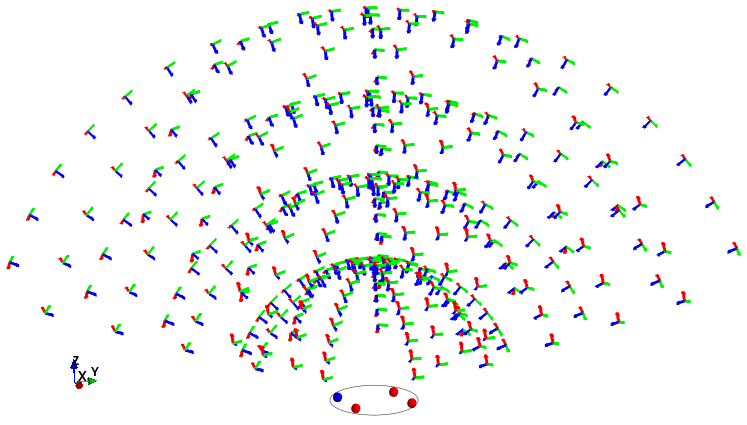
\includegraphics[width=\columnwidth]{img/cam_config3D.png}
			\caption{\label{fig:homography_results} \small Distribution of the 400 camera poses used in simulations. A circular plane with 4 control points inside the limits is displayed at the bottom. The circular plane lays on $z=0$ and its center is at the origin of the world coordinate system. The cameras are distributed evenly in spheres of different radius, each one looking at the center of the circular plane. Only camera poses which had the limits of the circular plane in field of view were used.}
		\end{center}
	\end{figure}
	Simulation description:
	
	
	Metrics for 3D rotatitons:\cite{Huynh2009}
	
	
	%%%%%%%%%%%%%FRONTO PARALLEL CASE
	%245.71811pt
	\begin{figure}[t]
		\begin{center}
			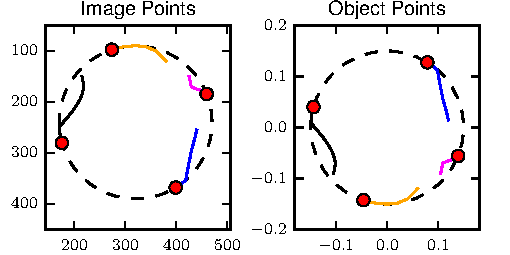
\includegraphics[width=\columnwidth]{img/image_control_points.pdf}
			\caption{\label{fig:homography_results} Movement of the points in image and object coordinates during gradient descent for the Fronto-Parallel configuration. The red dots mark the final point configuration.}
		\end{center}
	\end{figure}
	
	\begin{figure}[t]
		\begin{center}
			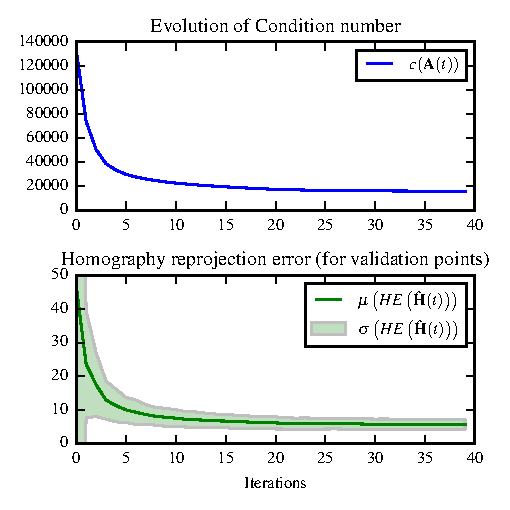
\includegraphics[width=\columnwidth]{img/homography_fronto_parallel.pdf}
			\caption{\label{fig:homography_results} Evolution of the condition number and the homography reprojection error during gradient descent (Fronto-Parallel configuration).}
		\end{center}
	\end{figure}
	
	\begin{figure}[t]
		\begin{center}
			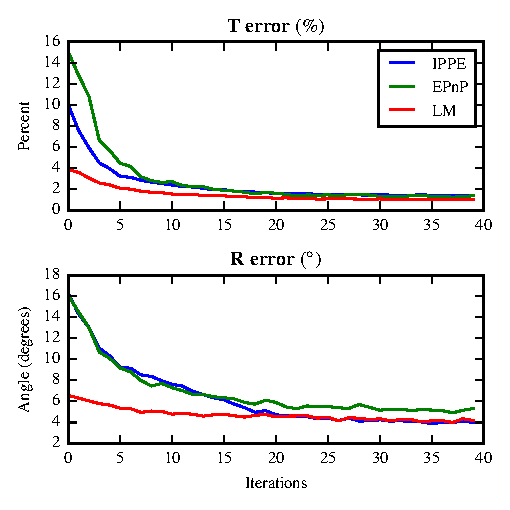
\includegraphics[width=\columnwidth]{img/pose_together_fronto_parallel.pdf}
			\caption{\label{fig:homography_results} Evolution of the pose estimation during gradient descent (Fronto-Parallel configuration).}
		\end{center}
	\end{figure}
	
	\begin{figure}[t]
		\begin{center}
			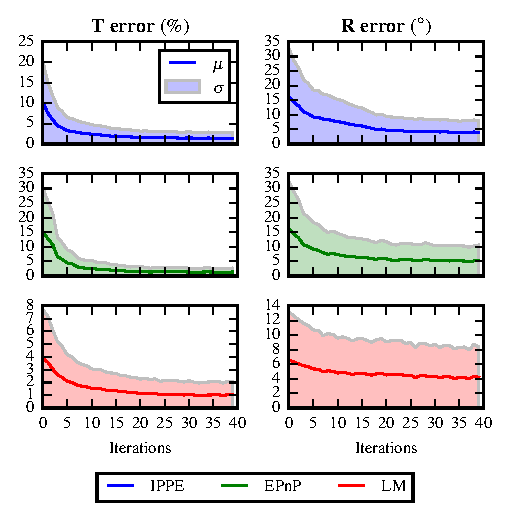
\includegraphics[width=\columnwidth]{img/pose_separate_fronto_parallel.pdf}
			\caption{\label{fig:homography_results} Evolution of the pose estimation during gradient descent for each algorithm including standard deviations (Fronto-Parallel configuration).}
		\end{center}
	\end{figure}
	
	
	%%%%%%%%%%%%%INCLINED CASE
	
	\begin{figure}[t]
		\begin{center}
			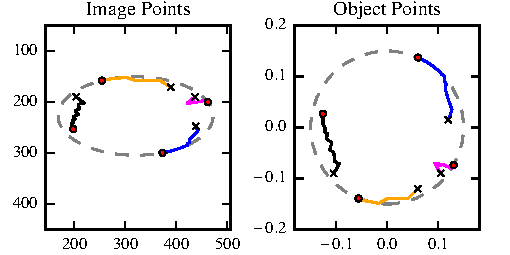
\includegraphics[width=\columnwidth]{img/image_control_points_inclined.pdf}
			\caption{\label{fig:homography_results} Movement of the points in image and object coordinates during gradient descent for the inclined configuration. The red dots mark the final point configuration.}
		\end{center}
	\end{figure}
	
	\begin{figure}[t]
		\begin{center}
			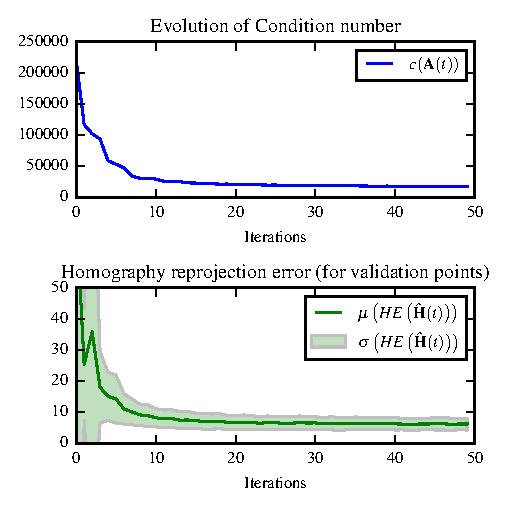
\includegraphics[width=\columnwidth]{img/homography_inclined.pdf}
			\caption{\label{fig:homography_results} Evolution of the condition number and the homography reprojection error during gradient descent (inclined configuration).}
		\end{center}
	\end{figure}
	
	\begin{figure}[t]
		\begin{center}
			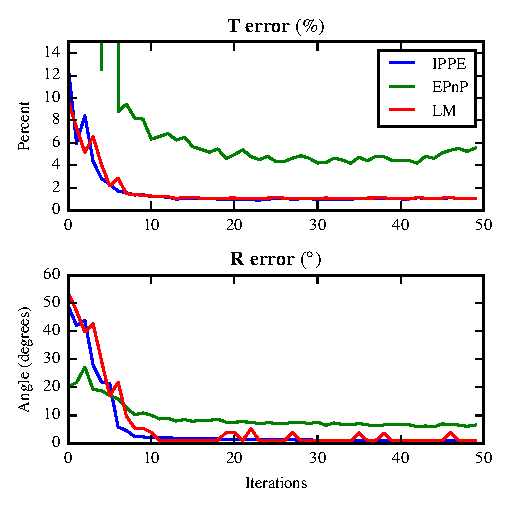
\includegraphics[width=\columnwidth]{img/pose_together_inclined.pdf}
			\caption{\label{fig:homography_results} Evolution of the pose estimation during gradient descent (inclined configuration).}
		\end{center}
	\end{figure}
	
	\begin{figure}[t]
		\begin{center}
			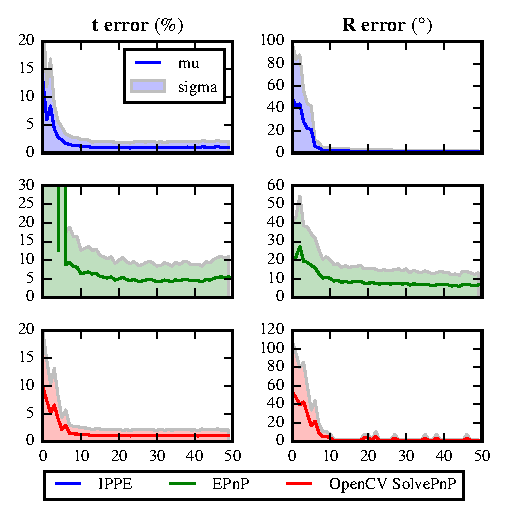
\includegraphics[width=\columnwidth]{img/pose_separate_inclined.pdf}
			\caption{\label{fig:homography_results} Evolution of the pose estimation during gradient descent for each algorithm including standard deviations (inclined configuration).}
		\end{center}
	\end{figure}
	
	
	%EFFECT OF WELL-CONDITIONED VS ILL-CONDITIONED POINT CONFIGURATIONS
	
	\begin{figure}[t]
		\begin{center}
			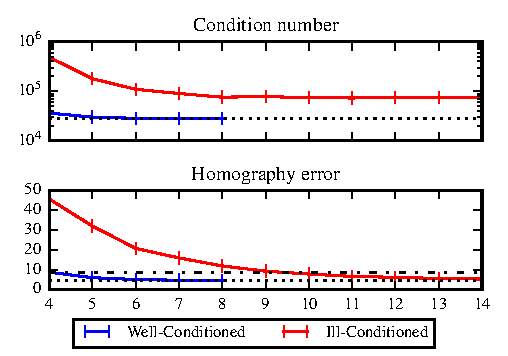
\includegraphics[width=\columnwidth]{img/point_config_comp_homo.pdf}
			\caption{\label{fig:homography_results} Well-conditioned point configurations in contrast to Ill-conditioned ones for Homography estimation.}
		\end{center}
	\end{figure}
	
	
	\begin{figure}[t]
		\begin{center}
			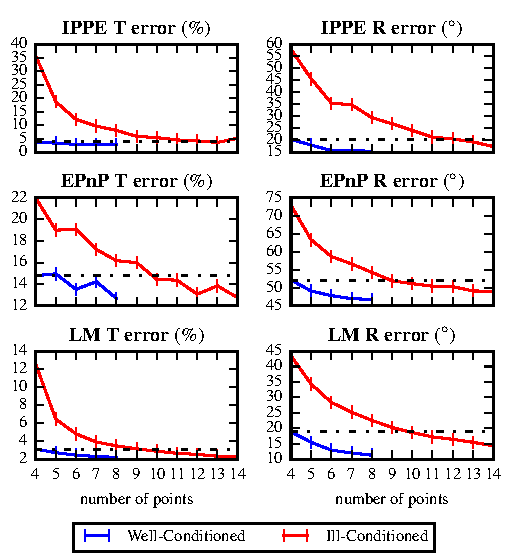
\includegraphics[width=\columnwidth]{img/point_config_comp_pose.pdf}
			\caption{\label{fig:homography_results} Well-conditioned point configurations in contrast to Ill-conditioned ones for Pose estimation..}
		\end{center}
	\end{figure}
	
	
	\todo[inline]{END OF RAUL'S PROTECTED ZONE. CONCLUSIONS ARE SAFE TO EDIT IF YOU WANT TO ADD SOMETHING.}
	
	\section{Conclusions and future work}
	\label{Conc}
	Mention that EPNP is considered not good for less that 6 points, but when we use the ideal point configuration for the pose then the results with 4 points are equally good.
	
	%\todo[inline]{Volker, fix the conclusion or we do it together}
	
	%\addtolength{\textheight}{-12cm}   % This command serves to balance the column lengths
	% on the last page of the document manually. It shortens
	% the textheight of the last page by a suitable amount.
	% This command does not take effect until the next page
	% so it should come on the page before the last. Make
	% sure that you do not shorten the textheight too much.
	
	%%%%%%%%%%%%%%%%%%%%%%%%%%%%%%%%%%%%%%%%%%%%%%%%%%%%%%%%%%%%%%%%%%%%%%%%%%%%%%%%
	
	
	
	%%%%%%%%%%%%%%%%%%%%%%%%%%%%%%%%%%%%%%%%%%%%%%%%%%%%%%%%%%%%%%%%%%%%%%%%%%%%%%%%
	
	
	
	%%%%%%%%%%%%%%%%%%%%%%%%%%%%%%%%%%%%%%%%%%%%%%%%%%%%%%%%%%%%%%%%%%%%%%%%%%%%%%%%
	%%%%%%%%%%%%%%%%%%%%%%%%%%%%%%%%%%%%%%%%%%%%%%%%%%%%%%%%%%%%%%%%%%%%%%%%%%%%%%%%
	%\section*{Acknowledgements}
	
	{\small
		\bibliography{IEEEabrv,bib_icra2018}
		
		@techreport{Stewart1998,
			title={Perturbation theory for the singular value decomposition},
			author={Stewart, Gilbert W},
			year={1998}
		}
		
	}
\end{document}


